\section{Introduzione}

\subsection{Descrizione del problema}
\label{descrizione_min_cut}
In questa relazione illustreremo dei confronti tra due algoritmi per risolvere il problema del \textbf{Minimum Cut}, confrontando i tempi di calcolo e la correttezza delle soluzioni trovate. \\
Quello del \textit{Minimum Cut} è un problema di ottimizzazione che può essere definito come segue:
\begin{center}
    \centering
    \textit{
        Dato un multigrafo $\mathcal{G}=(\mathcal{V}, \mathcal{E})$, trovare un insieme $\mathcal{E}{}'\subseteq \mathcal{E}$ tale che $\mathcal{E}{}'$ sia minimo,\\ ossia contenga il minor numero di archi.
    }
\end{center}
Nel caso specifico di questo laboratorio, il problema è stato esteso a grafi pesati; 
il problema diventa pertanto trovare l'insieme di lati da rimuovere da un grafo in 
modo tale che la somma dei pesi di questi sia minima, ovvero, determinare un 
\textit{taglio} $(S,T)$ di peso minimo per $\mathcal{G}$. Il peso del taglio è definito 
come: 
\[
    w(S,T) = \sum_{e \in E(S,T)} w(e)
\]
Per risolvere questo problema abbiamo implementato due algoritmi: l'algoritmo di \textit{Stoer e Wagner} e l'algoritmo di \textit{Karger e Stein}. Nello specifico, il primo è un algoritmo deterministico, mentre il secondo è un algoritmo randomizzato.

\subsection{Definizioni utili}

\subsubsection*{Multigrafo non orientato}
Un \textit{multigrafo} è un grafo $\mathcal{G}=(\mathcal{V}, \mathcal{E})$ tale che $\mathcal{V} \subseteq \mathbb{N}$, con $\mathcal{V}$ finito, e $\mathcal{E}$ è un multiinsieme a elementi del tipo $\{u, v\}: u\neq v$

\subsubsection*{Cammino in un multigrafo}
Un \textit{cammino in un multigrafo} consiste in una sequenza di nodi $\{v_1, v_2, ..., v_t\}$ dove per ogni coppia di nodi $\{v_i, v_{i+1}\}$ esiste un lato $e_j$ che li unisce.

\subsubsection*{Connettività di un multigrafo}
Un multigrafo è \textit{connesso} se per ogni coppia di nodi $v_i, v_j$ esiste un cammino che li connette.

\subsubsection*{Taglio}
Dato $\mathcal{G}=(\mathcal{V}, \mathcal{E})$ un multigrafo connesso, un \textit{taglio} $\mathcal{C} \subseteq \mathcal{E}$ è un multiinsieme di lati tale che $\mathcal{G}{}'=(\mathcal{V}, \mathcal{E}-\mathcal{C})$ non è connesso o, equivalentemente, $\mathcal{G}{}'$ ha almeno due componenti connesse.

\subsubsection*{Contrazione di un multigrafo rispetto ad \textit{e}}
\label{definizione_contrazione}
Dato $\mathcal{G}=(\mathcal{V}, \mathcal{E})$ un multigrafo ed $e=\{u,v\} \in \mathcal{E}$, la \textit{contrazione} di $\mathcal{G}$ rispetto ad $e$, $\mathcal{G}/e=(\mathcal{V}{}', \mathcal{E}{}')$ è il multigrafo con:
\begin{itemize}
    \item[] $\mathcal{V}{}'=\mathcal{V} \setminus \{u, v\} \cup \{z_{u,v}\}$
    \item[] $\mathcal{E}{}'=\mathcal{E} \setminus \{\{\{x, y\}: (x=u) \vee (x=v)\}\} \cup \{\{\{z_{u,v}, y\}: (\{u,y\} \in \mathcal{E}) \vee (\{v,y\} \in \mathcal{E}), (y\neq u) \wedge (y \neq v) \}\}$ % im dead inside 
\end{itemize}
Quando vengono contratti due vertici, viene eliminato il lato tra loro e 
si crea un nuovo vertice che li comprende, ereditando tutti i loro vecchi lati 
incidenti. Si osservi che:
\begin{enumerate}
    \item $|\mathcal{V}'| = |\mathcal{V}| - 1$ ($= |\mathcal{V}| - 2 + 1$);
    \item $|\mathcal{E}'| = |\mathcal{E}| - m(e) \le |\mathcal{E}| - 1$, ovvero, viene 
    rimosso almeno il lato che collega i due vertici da contrarre. $m(\cdot)$ è la 
    \textit{molteplicità}, ovvero, indica quante copie ci sono di un certo oggetto.
\end{enumerate}

Viene riportato di seguito un esempio grafico di contrazione di un multigrafo rispetto a un arco.

\begin{figure}[H]
	\centering
	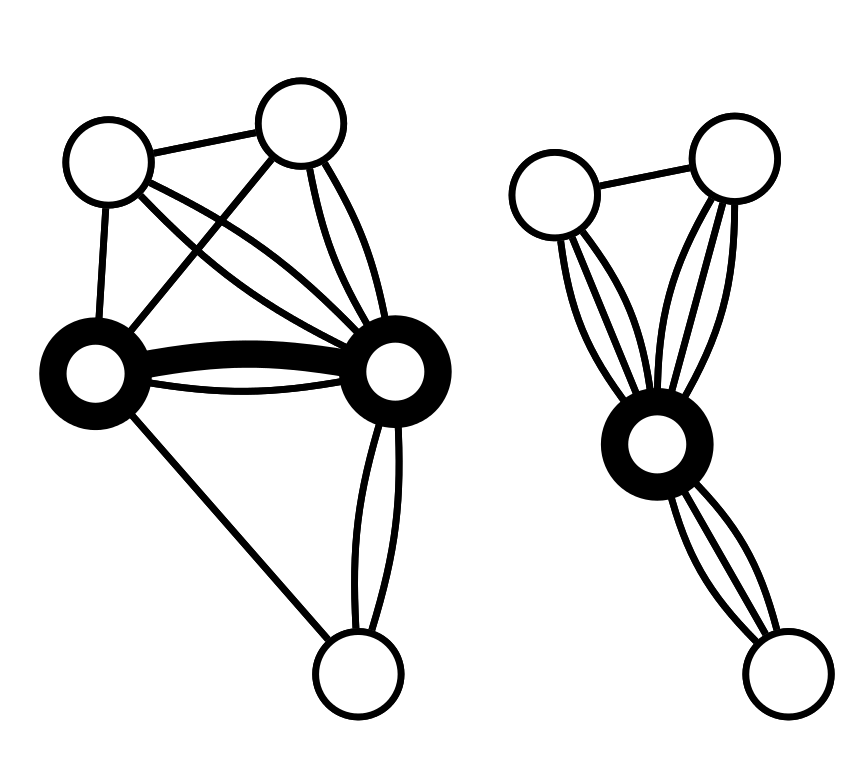
\includegraphics[width=0.5\textwidth]{res/images/multigraph}
	\caption{Esempio di contrazione di un multigrafo.}
	\label{fig:multigraph_contraction}
\end{figure}

\subsubsection*{Alta probabilità}

Ai fini dell'analisi dell'algoritmo di \textit{Karger} e \textit{Stein}, si forniscono le seguenti definizioni:
\begin{enumerate}
    \item \textbf{Alta probabilità}: dato $\Pi \subseteq \mathcal{I} \times \mathcal{S}$, dove $\Pi$ è un 
    \textit{problema decisionale}, un algoritmo $\mathcal{A}_{\Pi}$ ha complessità 
    $\mathcal{T}(n) = \mathcal{O}(f(n))$ con \textit{alta probabilità} se $\exists c, d > 0$ tali che 
    $\forall i \in \mathcal{I}$, $|i| = n$, $Pr(\mathcal{A}_{\Pi}(i)$ termina in $\ge c \dot f(n)$ passi $) \le \frac{1}{n^d}$, 
    ovvero, la probabilità che l'algoritmo superi la complessità $\mathcal{O}(f(n))$ è molto bassa $\Bigl(\frac{1}{n^d}\Bigr)$.
    \item \textbf{Correttezza con alta probabilità di un algoritmo}: dato $\Pi \subseteq \mathcal{I} \times \mathcal{S}$, 
    un algoritmo $\mathcal{A}_{\Pi}$ è corretto con alta probabilità se $\exists d > 0$ tali che 
    $\forall i \in \mathcal{I}$, $|i| = n$, $Pr((i, \mathcal{A}_{\Pi}) \notin \Pi) \le \frac{1}{n^d}$.
\end{enumerate}

\subsubsection*{Introduzione agli algoritmi randomizzati}
Un algoritmo randomizzato è un algoritmo che include un certo grado di 
\textit{casualità}. Il comportamento di un algoritmo randomizzato non è determinato 
unicamente dall'input, ma dipende anche da un certo fattore casuale. Le prestazioni 
dell'algoritmo, inclusi il tempo di esecuzione o l'output, saranno a loro volta casuali.
Tipicamente l'algoritmo utilizza variabili aleatorie come input ausiliario 
per guidare il suo comportamento con l'obiettivo di ottenere, in media, buone 
prestazioni. In base all'utilizzo che viene fatto delle variabili 
casuali, l'algoritmo può essere progettato per restituire sempre la risposta corretta 
(\textit{algoritmo Las Vegas}), a scapito del tempo di calcolo, o per prevedere 
anche che il risultato calcolato possa essere errato con una certa probabilità 
(\textit{algoritmo Monte Carlo}). Una volta che il fattore casuale è stato ottenuto, 
il comportamento dell'algoritmo risulta determinato unicamente dall'input e quindi 
esso può essere visto come un algoritmo deterministico.

\subsubsection*{Algoritmi Las Vegas}
In questa categoria sono compresi tutti gli algoritmi randomizzati che restituiscono 
sempre la soluzione corretta.
\[
    \forall i \in \mathcal{I}, \mathcal{A}_{R}(i) = s:(i,s) \in \Pi
\]

dove $\Pi \subset \mathcal{I} \times \mathcal{S}$ rappresenta il 
\textit{problema decisionale}, $i \in \mathcal{I}$ è un input, $\mathcal{I}$ è 
l'insieme di input, $\mathcal{S}$ è l'insieme delle soluzioni, 
$\mathcal{A}_{R}(i) = s$ è un algoritmo randomico che, applicato all'istanza di 
input $i$, produce una soluzione $s$ tale che la coppia $(i,s) \in \Pi$. Ovvero, 
$s$ è una soluzione dell'istanza $i$ del problema decisionale $\Pi$ ($s$ non è 
sempre la stessa $\forall i$). La randomizzazione è sfruttata nell'analisi della 
complessità dell'algoritmo. $\forall n, \mathcal{T}(n)$ è una variabile aleatoria di 
cui si studia:
\begin{enumerate}
    \item $E[\mathcal{T}(n)]$ oppure
    \item $Pr(\mathcal{T}(n) \ge c \cdot f(n)) \le \frac{1}{n^k}$ 
    \textit{alta probabilità}. Se si riesce a dimostrare questo, allora si dice che 
    l'algoritmo ha una complessità $\mathcal{O}(f(n))$ con alta probabilità.
\end{enumerate}

Lo spazio di probabilità corrisponde alle scelte casuali operate dall'algoritmo, da 
non confondere con l'analisi probabilistica di un algoritmo deterministico, dove lo 
spazio di probabilità coincide con la distribuzione degli input.

\subsubsection*{Algoritmi Monte Carlo}
Data un'istanza di input, è possibile che l'output dell'algoritmo su quell'istanza 
sia una soluzione $s$ che non è una soluzione corretta:
\[
    \exists i \in \mathcal{I}, \mathcal{A}_{R}(i) = s:(i,s) \notin \Pi
\]

Con questo tipo di algoritmi, quello che si studia è $Pr((i,s) \notin \Pi)$ in 
funzione di $|i| = n$. Si ha una famiglia di variabili aleatorie \textit{binarie} che 
rappresentano il fatto che l'algoritmo sia corretto o meno (una variabile $\forall$ 
input). Anche il tempo $\mathcal{T}(n)$ potrebbe essere una variabile aleatoria.

Questa categoria di algoritmi per i problemi decisionali si dividono in:
\begin{enumerate}
    \item \textit{one-sided}: l'algoritmo sbaglia soltanto su una singola risposta. 
    Ad esempio, l'algoritmo fa giuste tutte le istanze \verb|Si|, ma può sbagliare 
    le istanze del \verb|No|;
    \item \textit{two-sided}: l'algoritmo sbaglia in entrambe le risposte. L'algoritmo 
    può sbagliare sia sulle istanze del \verb|Si| che del \verb|No|.
\end{enumerate}